%&latex
%
\documentclass[../template.tex]{subfiles}
\begin{document}

\chapter{MoTP Baiesi Exercises 2019/20}

\section{Lesson 2}
\begin{exo}[Fourier transform of derivative]
    Show that the following formula holds for the Fourier transform ($\mathcal{F}(f) = \tilde{f}(k)$) of a derivative of the function $f(x)$ (under the usual mathematical assumptions for having a Fourier transform and its derivative):
    \begin{align*}
        \mathcal{F}\left(\dv{x} \theta(x)\right) = i k \tilde{f}(k)
    \end{align*}
    \medskip
    \textbf{Solution}. 
    \begin{align*}
        \mathcal{F}\left[\dv{x} f(x)\right](k) = \int_{\mathbb{R}} \dd{x} (\partial_x f(x)) e^{-ikx} \underset{(a)}{=} \cancel{e^{ikx} f(x) \Big|_{x=-\infty}^{x=+\infty} }+ ik \int_{\mathbb{R}} \dd{x} e^{ikx} f(x) = ik\tilde{f}(k)
    \end{align*}
    where in (a) we performed an integration by parts. The boundary term vanishes because we assume $f, f' \in L^2(\mathbb{R})$ to be able to compute their Fourier transform, so that $f(x) \to 0$ for $|x| \to \infty$.
\end{exo}

\begin{exo}[Fourier transform of $1$]
    Show that $\mathcal{F}(1) = 2 \pi \delta (k)$.
    \medskip

    \textbf{Solution}. By applying the definition of the $\delta(k)$ distribution:
    \begin{align*}
        \mathbb{F}[1](k) = \textcolor{Red}{2\pi} \underbrace{\int_{\mathbb{R}} \dd{x} \frac{e^{-ikx}}{\textcolor{Red}{2 \pi}}}_{ \delta(k)}   = 2\pi \delta(k)
    \end{align*}
    Alternatively, we can show that:
    \begin{align*}
        \mathcal{F}^{-1}[2 \pi \delta(k)](x) = \int_{\mathbb{R}} \frac{2\pi}{2\pi} e^{ikx} \delta(k) \dd{k} \underset{(a)}{=}  e^{i0x} = 1 
    \end{align*}
    where in (a) we applied $\langle \delta, f \rangle = f(0)$.
\end{exo}
\begin{figure}[H]
    \centering
    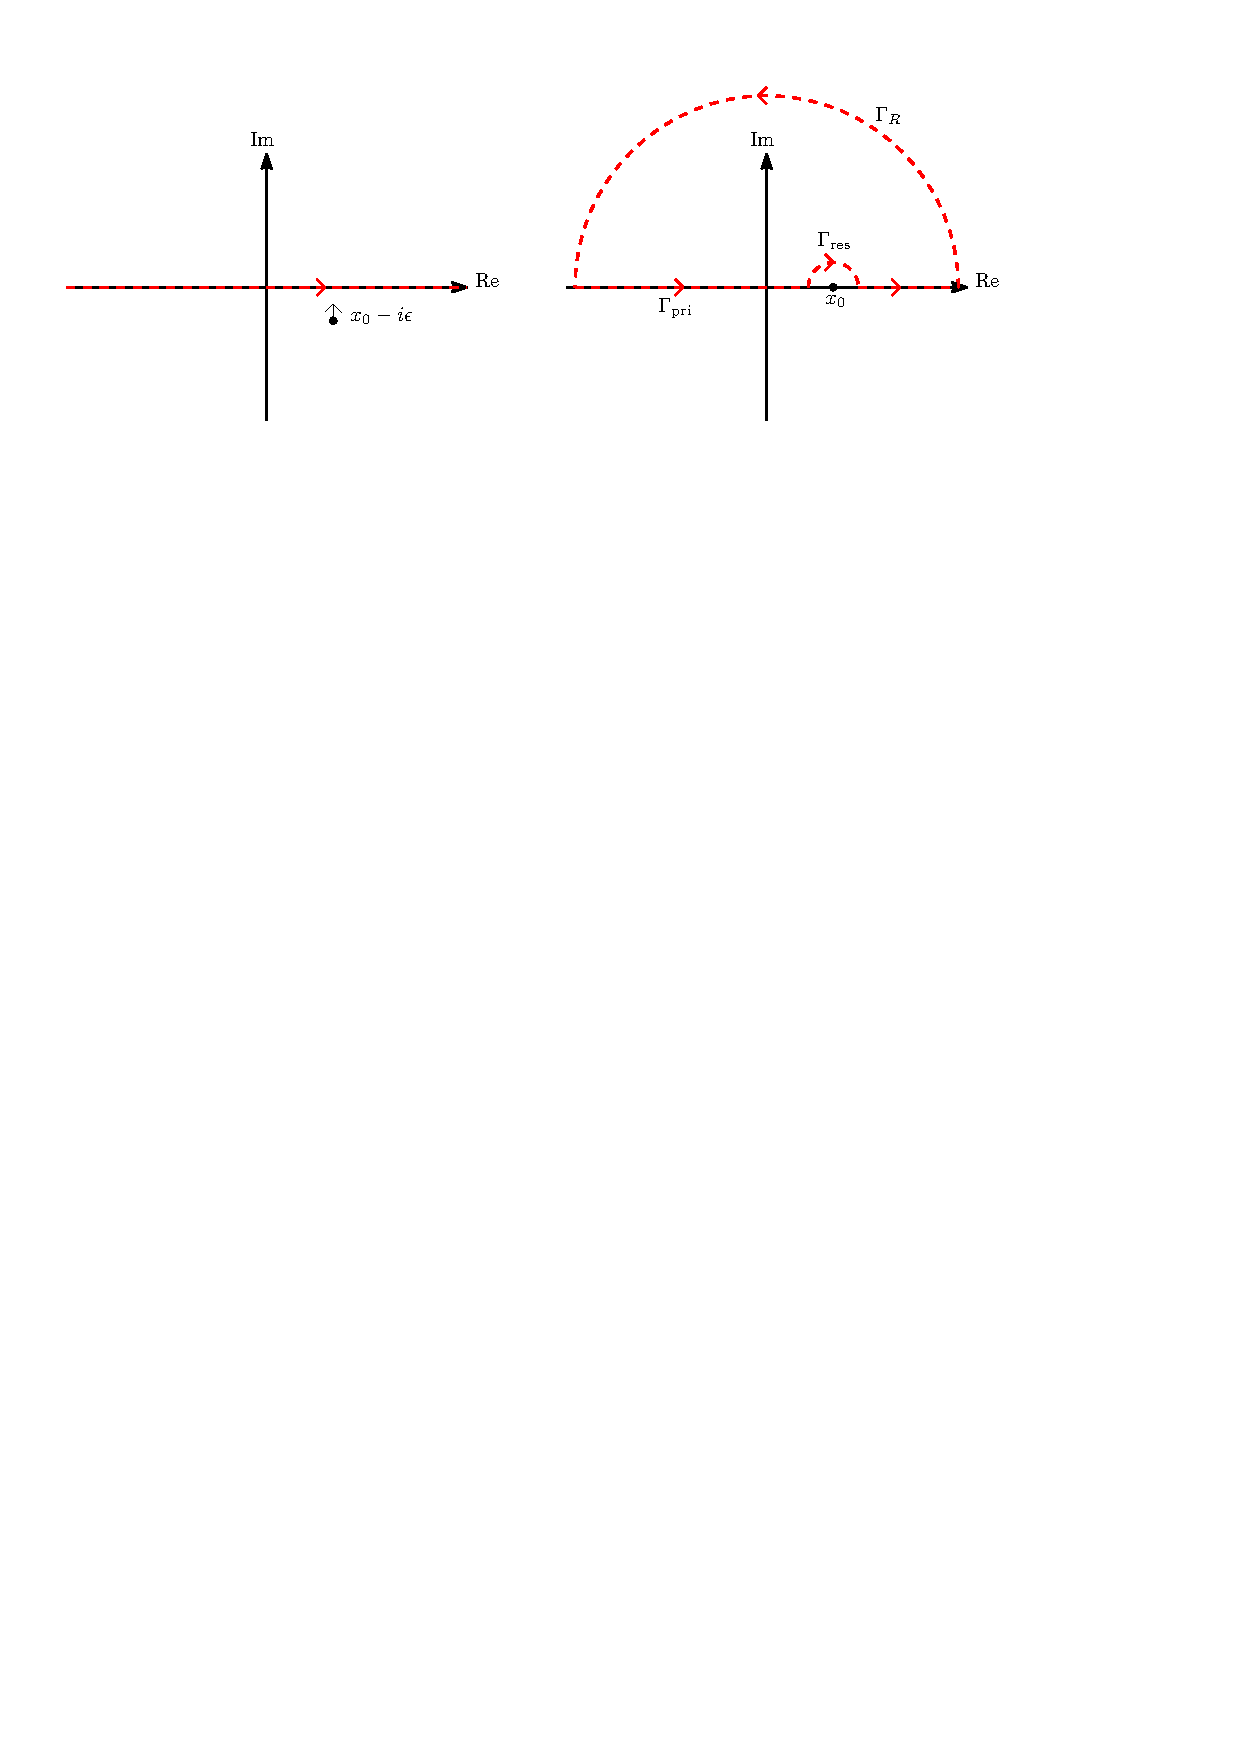
\includegraphics{Images/residue_int.pdf}
    \caption{\textbf{Left}: integral on the real line with approaching singularity. \textbf{Right}: integral using a closed curve and a shifted singularity.\label{fig:residue}}
\end{figure}
\begin{exo}[Prescription $i \epsilon$]
    To complete the case discussed during the lecture, compute:
    \begin{align*}
        \lim_{\epsilon \to 0} \frac{1}{x - x_0 + i \epsilon} = P\left[\frac{1}{x - x_0 } \right] - i \pi \delta (x - x_0 )
    \end{align*}
    Note that this limit and that discussed in the lecture are a physicists' crude shorthand notation for the full equation:
    \begin{align*}
        \lim_{\epsilon \to 0^+} \int_{-\infty}^{+\infty} \frac{f(x)}{x - x_0 \mp i \epsilon} \dd{x} = P \int_{-\infty}^{+\infty} \frac{f(x)}{x- x_0} \dd{x} \pm i \pi f(x_0)  
    \end{align*}
    and $f(z) \to 0$ for $|z| \to \infty$ and analytic in the $\operatorname{Im}(z) \geq 0$ portion of the complex plane.
    
    \medskip

    \textbf{Solution}. The integral on the real line with an approaching singularity from $\operatorname{Im}(z) \leq 0$ (figure \ref{fig:residue}, left) can be computed by using the closed curve shown in (figure \ref{fig:residue}, right), and applying Cauchy's integral theorem.
    The integrand, extended to the complex plane, is:
    \begin{align*}
        g(z) = \frac{f(z)}{z - (x_0 - i \epsilon)} 
    \end{align*}
    By hypothesis, the integral over $\Gamma_R$ vanishes:
    \begin{align*}
        \int_{\Gamma_R} g(z) \dd{z} = 0
    \end{align*}
    Then, the integral over $\Gamma_{\mathrm{pri}}$ is, by definition, the principal part of the real integral:
    \begin{align*}
        \int_{\Gamma_{\mathrm{pri} }} g(z) \dd{z} = P \int_{\mathbb{R}} \dd{x} \frac{f(x)}{x-x_0} 
    \end{align*}
    And finally, the integral over $\Gamma_{\mathrm{res}}$ is equal to half the residue at $x_0$, with a minus sign given by the clockwise rotation:
    \begin{align*}
        \int_{\Gamma_{\mathrm{res}}} g(z) \dd{z} = - \frac{2\pi i}{2} f(x_0) = - \pi i f(x_0) 
    \end{align*}
    This proves the required relation:
    \begin{align*}
        \lim_{\epsilon \to 0^+} \int_{\mathbb{R}} \frac{f(x)}{x - x_0 + i \epsilon} \dd{x} = P \int_{\mathbb{R}} \dd{x} \frac{f(x)}{x- x_0} - i \pi f(x_0)  
    \end{align*}
\end{exo}

\begin{figure}[H]
    \centering
    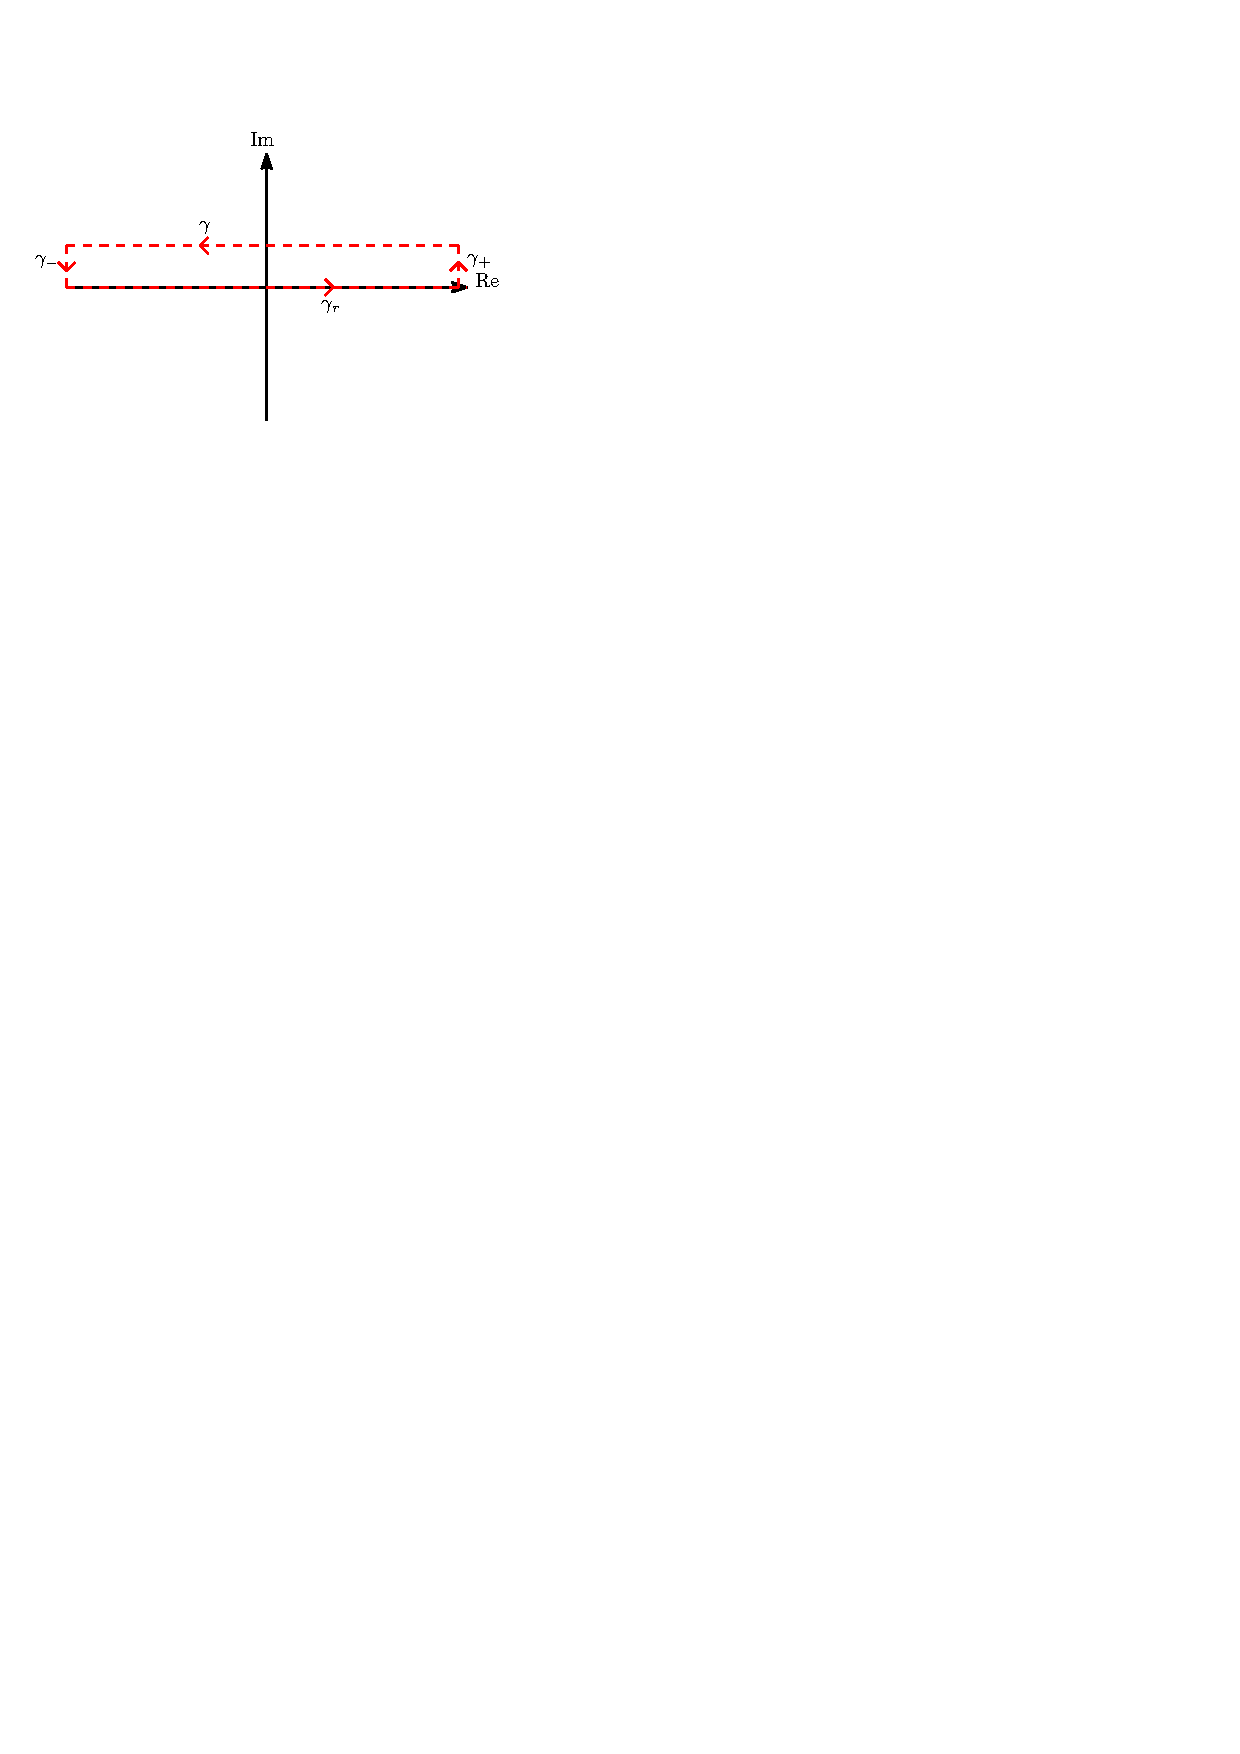
\includegraphics{Images/residue_int2.pdf}
    \caption{Closed path for the gaussian integral.\label{fig:residue2}}
\end{figure}

\begin{exo}[Gaussian integral]
    Compute the Gaussian integral
    \begin{align*}
        I = \int_{-\infty}^{\infty} \dd{x} \exp(-ax^2 + bx) = \sqrt{\frac{\pi}{a} } \exp\left(\frac{b^2}{4a} \right)
    \end{align*}
    for $a \in \mathbb{R}, a > 0$ and complex $b = \beta + i \nu$ (with $\beta, \nu \in \mathbb{R}$). For the solution, one may shift to a new variable $z$ with $x=z+iq$, so that the exponent in the integral does not contain a term $\sim iz$ and the new path of integration can be mapped back to the real axis by using Cauchy's theorem.
\medskip

    \textbf{Solution}. The starting integral is:
    \begin{align*}
        I = \int_{\mathbb{R}} \dd{x} \exp(-ax^2 + \beta x + i \nu x)
    \end{align*}
    We then perform a change of variables:
    \begin{align*}
        x = z + iq \Rightarrow \dd{x} = \dd{z}
    \end{align*}
    moving the integral from the real line to $\gamma$, i.e. the horizontal line at $\operatorname{Im} z  = iq$.
    \begin{align*}
        I = \int_\gamma \dd{z} \exp(-a(z+iq)^2 + \beta(z+iq) + i \nu (z + iq) )
    \end{align*}
    Expanding the exponential argument leads to:
    \begin{align*}
        -a(z^2 - q^2 + 2iqz) + \beta z + i \beta q + i \nu z - \nu q =\\
        -az^2 + z \beta + iz(\nu - 2 qa) + a q^2 - \nu q + i \beta q
    \end{align*}
    To remove the $iz$ term we set $\nu - 2 qa = 0 \Rightarrow q = \nu/(2a)$, leading to:
    \begin{align*}
        = -az^2 + z \beta + \frac{a \nu^2}{4 a^2} - \frac{\nu^2}{2a} + i\frac{\beta \nu}{2a} = -az^2 + z \beta -\frac{\nu^2}{4a} + i\frac{\beta \nu}{2a}     
    \end{align*}
    Substituting back in the integral:
    \begin{align*}
        I = \int_{\gamma} \dd{z} \exp(-az^2 + z \beta) \exp\left(-\frac{\nu^2}{2a} + i \frac{\beta \nu}{2a}  \right)
    \end{align*}
    Consider now the closed path shown in fig. \ref{fig:residue2}. In the limit where $\gamma_r$ goes from $-\infty$ to $+\infty$, the integrals over $\gamma_+$ and $\gamma_-$ vanish, as $\exp(-az^2+bz) \to 0$ for $|z| \to \infty$. Then, as the closed path does not contain any singularity, by Cauchy's integral theorem we have that the integral along $\gamma$ is the same as the integral on the real line (assuming the same orientation). This allows us to evaluate $I$ on the real line:
    \begin{align*}
        I = \int_{\mathbb{R}} \dd{x} \exp(-ax^2 + x \beta) \exp\left(-\frac{\nu^2}{2a} + i\frac{\beta \nu}{2a}  \right) &= \sqrt{\frac{\pi}{a}} \exp\left(\frac{\beta^2}{4a} - \frac{\nu^2}{4a} + i\frac{\beta \nu}{2a}   \right) =\\
        &= \sqrt{\frac{\pi}{a} } \exp\left(\frac{(\beta + i \nu)^2}{4a}  \right)= \sqrt{\frac{\pi}{a} } \exp\left(\frac{b^2}{4a} \right)
    \end{align*}
\end{exo}

\section{Lesson 3}
\begin{exo}[Cauchy distribution]
    Expand the details of these passages:
    \begin{align*}
        P(x, t)=\frac{1}{2 \pi} \int_{-\infty}^{\infty} \dd{k} e^{-x^{*}|k|+i k x}=\frac{1}{\pi} \int_{0}^{\infty} \dd{k} e^{-x^{*} k} \cos k x=\frac{1}{\pi x^{*}} \frac{1}{1+\left(\frac{x}{x^{*}}\right)^{2}}
    \end{align*}
    used to find the one-dimensional Cauchy distribution. Finding the last term by skipping entirely the $\cos kx$ step is also an option. Here $x=0$ at $t=0$ and $x^* = D_1t$.
    \medskip

\textbf{Solution}. We start from the \textit{generalized diffusion equation}:
\begin{align*}
    \begin{cases}
        \partial_t P(x,t) = D_\mu \pdv{|x|^\mu} P(x,t)\\
        P(x,0) = \rho(x)
    \end{cases}
\end{align*} 
with $0 < \mu < 2$. The \textit{fractional} derivative makes sense after passing in Fourier space:
\begin{align*}
    \partial_t \tilde{P}(k,t) = - D_{\mu}|k|^\mu \tilde{P}(k,t) \Leftrightarrow \partial_t[ \exp(D_\mu |k|^\mu t) \tilde{P}(k,t)] = 0
\end{align*} 
This means that the exponential must be time independent:
\begin{align*}
    \tilde{f}(k) \equiv \exp(D_{\mu} |k|^\mu t) \tilde{P}(k,t) \Rightarrow \tilde{P}(k,t) = \tilde{f}(k) \exp(-D_\mu |k|^\mu t)
\end{align*}
Since $\tilde{f}(k)$ so defined does not depend on time, we can compute it by setting $t=0$, leading to $\tilde{f}(k) = \tilde{P}(k,0) = \tilde{\rho}(k)$. 

Cauchy random flights are found by setting $\mu = 1$. The equation becomes:
\begin{align*}
    \tilde{P}_C(k,t) = \tilde{\rho}(k) \exp(-D_1 |k|t)
\end{align*}
Assuming that the particle is localized in $x=0$ at $t=0$, then $\rho(x) = \delta(x)$, and so $\tilde{\rho}(k) = \mathbb{F}[\delta(x)](k) = 1$, leading to:
\begin{align*}
    \tilde{P}_C(k,t) = e^{-D_1|k|t} = \exp(-x^*(t)|k|)
\end{align*}
To return to position space, we compute a Fourier anti-transform:
\begin{align*}
    P_C(x,t) &= \mathcal{F}^{-1} [\tilde{P}_C] (x,t) = \frac{1}{2\pi} \int_{\mathbb{R}} \dd{k} \exp(-x^*(t)|k| - ikx) = \\
    &=  \frac{1}{2\pi} \int_{\mathbb{R}} \dd{k} \textcolor{Red}{e^{-x^*(t)|k|}} \left[\textcolor{Red}{\cos(-kx)} + i \textcolor{Blue}{\sin(-kx)}\right] 
\end{align*}
Note that the domain is symmetric, and the red terms are even, while the blue one is odd. So the $\sin$ contribution will be $0$, leading to:
\begin{align*}
    P_C(x,t)= \frac{1}{2 \pi} 2 \int_0^{+\infty} \dd{k} e^{-x^*(t) k} \cos(kx) 
\end{align*}

The integral can be computed with a double integration by parts:
\begin{align*}
    I &= \int_0^{+\infty} e^{-x^* k} \cos(kx) \dd{k} = - \cos(kx) \frac{1}{x^*} e^{-x^*k} \Big|_{k=0}^{k=+\infty} + x \sin(kx) (x^*)^{-2} e^{-x^* k} \Big|_{k=0}^{k=+\infty}\\
    &\quad\> - \int_0^{+\infty}\dd{k} x^2 \cos(kx) (x^*)^{-2} e^{-x^* k} =\\
    &= \frac{1}{x^*} - \frac{x^2}{(x^*)^2}I \Rightarrow I = \frac{1}{x^*} \frac{1}{1+\left(\frac{x}{x^*} \right)^2}    
\end{align*}
And readding the $1/\pi$ factor leads to the desired solution:
\begin{align*}
    P_C(x,t) = \frac{1}{\pi x^*} \frac{1}{1+\left(\frac{x}{x^*} \right)^2}  
\end{align*}
\end{exo}

\begin{exo}[Transition probabilities and Cauchy flights]
    With the Cauchy jump distribution with typical displacement $x^{*}=D_{1} t$ at time $t$ (see previous exercise, setting $x=$ displacement), compute the probability $P(x, t)$ to find the particle at position $x$ at time $t$ for such a Levy process, when the initial distribution is uniform and bound as $P(x, 0)=\rho(x)=1 /(2 a)$ for $x \in[-a, a]$ and $\rho(x)=0$ otherwise.

    \medskip

    \textbf{Solution}. The initial distribution is given by:
    \begin{align*}
        P(x,0) = \rho(x) = \begin{cases}
            \frac{1}{2a} & x \in [-a,+a]\\
            0 & \text{otherwise} 
        \end{cases}
    \end{align*} 
    The probability of a particle being in $x$ at $t$ is obtained by \textit{propagating} the initial distribution:
    \begin{align*}
        P(x,t) &= \int_{\mathbb{R}} \dd{x_0} P(x,t|x_0,0) P(x_0,0) = \\
        &= \int_{-a}^{+a} \dd{x_0} \frac{1}{\pi x*} \frac{1}{1+\left(\frac{x- x_0}{x^*} \right)^2} \frac{1}{2a} = \\
        &= -\frac{1}{2 a \pi x^*(t)}   \arctan\left(\frac{x-x_0}{x^*} \right)\Big|_{x_0 = -a}^{x_0 = +a} =\\
        &= \frac{1}{2 \pi a x^*(t)} \left[-\arctan\left(\frac{x-a}{x^*} \right) + \arctan\left(\frac{x+a}{x^*} \right)\right] 
    \end{align*} 
\end{exo}

\begin{exo}[Numerical simulation - optional]
Check numerically that the sum $S_{n}=x_{1}+\ldots+x_{n}$ of $n$ i.i.d. variables $x \in \mathbb{R},$ each one distributed according to
$$
p(x)=\frac{1}{4 x^{2}} \quad \text { for }|x|>1, \quad p(x)=1 / 4 \text { for }|x| \leq 1
$$
converges to a Cauchy distribution
$$
P_{\text {Cauchy }}(Y)=\frac{1}{\pi\left(1+Y^{2}\right)}
$$
after a suitable rescaling $Y_{n}=\gamma S_{n} / n^{\beta} .$ What are $\gamma$ and $\beta ?$
\end{exo}

See the Jupyter notebook at this link: \url{https://github.com/Einlar/data_notes/blob/revision/Models/Plots/Baiesi3_3-simulation.ipynb}.
\end{document}
